\chapter{Implementation}
\label{ch:implementation}
\acresetall

This chapter goes into depth on how the design from the previous chapter is
implemented into the BATMAN protocol. Some code snippets will be shown in the
following sections when applicable, and the full source code can be found in
Appendix \ref{appendix:source}.

%\begin{figure}[h]
%	\centering
%	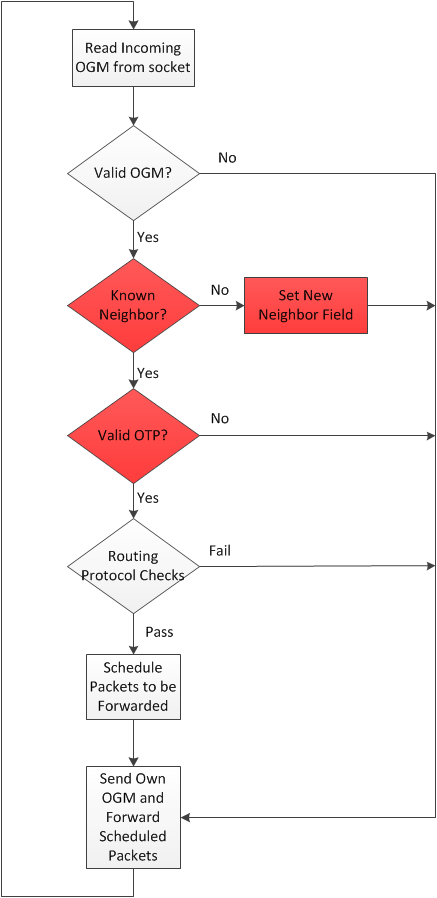
\includegraphics[totalheight=1\textheight]{images/batman_if_statements.png}
%	\caption{IF-Statements in the Batman Class}
%	\label{fig:batman_if_statements}
%\end{figure}

\section{Authentication Module}
Almost all functionality added to BATMAN is within the borders of a separate
class called \ac{AM}. The first thing to notice about the \ac{AM} is that it
runs in its own thread and sockets, so all authentication mechanisms run
concurrent to regular BATMAN routing operations. This separation was necessary
in order to have BATMAN behave normally during e.g. the authentication of a
node, so a large network should not suffer if an important node (centrally
located) is 'hung up' in e.g. authenticating another node.

\subsection{AM Thread}
In the setup phase in the original batman class, an \ac{AM} initiation function
called \texttt{am\_thread\_init} from the \ac{AM} class is called. This function
takes the network interface name and its corresponding IP address and broadcast
address as input. These values are then stored locally in in the AM class for
socket setup. For socket setup see Section \ref{subsect:am_socks}.

The function then goes on to create a new thread for the AM module which is the
main thread taking care of most of the additions in this implementation. The
thread first sets up two sockets for sending and receiving AM messages such as
handshakes and keystream-materials.

Next it generates a highly random (high entropy) master key using the OpenSSL
function \texttt{RAND\_bytes}, which has been properly seeded - see Section
\ref{subsect:posix.c}. This and an IV generated with OpenSSL's
\texttt{RAND\_pseudo\_bytes} is then used to generate a master key encryption
context for AES encryption, before deleting the master key. With the encryption
context the necessary internal memory used by OpenSSL for encrypting with this
key is stored, and therefore the key and IV is of no more use by themselves -
making it a sound security choice to delete the key (and IV) entirely.

The next important action is to generate either a \ac{PC0} or a \ac{PC} request
depending on whether you are a \ac{SP} or just a regular node trying to
authenticate with the network.

After these steps the ``initiation phase'' of the AM thread is complete, and the
rest of the code runs in a loop until the BATMAN daemon is terminated.

\subsection{AM Sockets}\label{subsect:am_socks}
Two sockets are used for the AM module, one for sending and one for receiving AM
messages. Both sockets are bound to the interface device given by the AM
initiation function. The receive socket is then bound to a designated port
64305, regular BATMAN runs on port 4305, and the send socket is explicitly
allowed to send to broadcast addresses.

Sockets needs to be explicitly set to be allowed to send to broadcast addresses
in UNIX systems, as a protection mechanism.

The following shows a code snippet of how the sockets are setup:
\begin{lstlisting}[frame=tb]
int32_t *recvsock, *sendsock;
addrinfo hints, *res;

/* Set family information */
memset(&hints, 0, sizeof hints);
hints.ai_family = AF_INET;
hints.ai_socktype = SOCK_DGRAM;
hints.ai_flags = AI_PASSIVE;
hints.ai_protocol = IPPROTO_UDP;

/* Puts the port-info inside a addrinfo data structure */
getaddrinfo(NULL, port, &hints, &res);

/* Assign file descriptor for sockets */
*recvsock = socket(PF_INET, SOCK_DGRAM, 0)
*sendsock = socket(PF_INET, SOCK_DGRAM, 0)

/* Binds the sockets to the network interface */
setsockopt(*recvsock, SOL_SOCKET, SO_BINDTODEVICE, interface, strlen(interface) + 1)
setsockopt(*sendsock, SOL_SOCKET, SO_BINDTODEVICE, interface, strlen(interface) + 1)

/* Binds receive socket to the port (rest of the address is empty/null) */
bind(*recvsock, res->ai_addr, res->ai_addrlen);

/* Allow the send socket to send broadcast messages */
int broadcast_val = 1;
setsockopt(*sendsock, SOL_SOCKET, SO_BROADCAST, &broadcast_val, sizeof int)

/* Set the send socket to non-blocking */
fcntl(*sendsock, F_SETFL, O_NONBLOCK);

\end{lstlisting}

There are several practical reasons to choose UDP sockets over TCP sockets for
this implementation. First and foremost, this system sends authentication
handshake messages and keystream-material messages to nodes which has no route
in the routing tables. If a connection-oriented protocol would try this the
messages would be blocked on the kernel level and not sent. With an
connectionless protocol like UDP no mechanisms will block this message being
sent, it will just send the message not bothering whether the message is ever
received by the recipient.

Second, TCP was created with wired networks in mind, observing much less packet
loss. In \acp{MANET} the packet losses are much higher than in wired and fixed
infrastructure networks, and as nodes move around direct paths between nodes
change much more frequently. TCP is not suitable for such environments because
it will lead to a huge amount of re-sending of packets to ``non-existant''
neighbors and much memory wasted in connection states being kept for dead links.

\subsection{Main Operation of the AM Thread}
Most of the interesting operation in the AM class happens within a single loop
running throughout the lifetime of the BATMAN daemon. The program flow
throughout this loop is shown in Figure \ref{fig:am_main_loop}.

\begin{figure}[hb!]
	\centering
	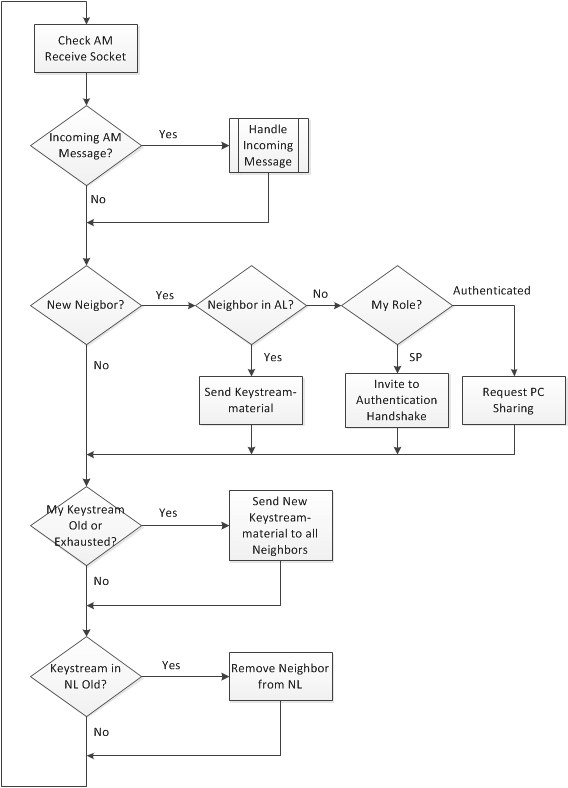
\includegraphics[width=\textwidth]{images/am_main_loop.png}
	\caption{Main program flow in AM class.}
	\label{fig:am_main_loop}
\end{figure}

For clarity the figure leaves out certain details, but the most important
features are depicted. The handle incoming messages are shown as a sub-process
in the figure.  This is not true, but depicting all possible messages would not
fit the figure, and therefore left out altogether. However, each message are
described in the following sections.

The ``New Neighbor'' is one of the elements in the AM class that must be
triggered by the batman class. If the batman thread tells the AM thread a new
neighbor is discovered and the AM thread is in a ready state to handle new
neighbors the appropriate action is taken, whether the neighbor has been
authenticated with the network or not. Not shown in the figure is how a regular
authenticated node will act if a new neighbor which is not authenticated with
the network is handled, but this is taken care of in the batman class and not
here.

The two last parts should be self-explanatory, they simply check the current
time and then compares this against time values set on the nodes own current
keystream to check if its old, or if any keystreams from other neighbors in the
\ac{NL} are old and if so takes the appropriate action. Also checked is if a
nodes own keystream is getting exhausted, in which also the appropriate action,
namely creating and sharing a new one with each neighbor in the \ac{NL}.


\section{Proxy Certificates}
The \acp{PC} in this implementation are containers for short lived 1024 bits RSA
public keys used in a single session only. Most of the design choices were taken
into the implementation, but some however, were left due to time constraint.

One such was that the original proxy certificate X.509v3 extension, introduced
in RFC 3820 called ``proxyCertInfoExtension'' was not used to carry the policies as
intented. Most of the OpenSSL documentation is not released to the general
public for free, and this X.509v3 extension was no exception. The only examples
found, amongst the original proxy certificate implementations from the Globus
Project\footnote{Globus Project:
\url{http://www.globus.org/toolkit/downloads/}}, but using the exact same setup
did not work in my implementation. After some investigation it seems no open
source code projects using proxy certificates have been publiished for years,
giving me the idea that maybe the OpenSSL specifications have changed during
the last version updates and that proxy certificates have to be implemented
differently. The author have asked for an answer on this subject on both emails
to the developers of OpenSSL, the OpenSSL's mailinglists, and on an
OpenSSL ``IRC'' channel\footnote{OpenSSL IRC Channel: \#openssl on
\url{irc://irc.freenode.net}}.

As a replacement for this extension, a commonly used free-text extension called
\texttt{netscape\_comment} has been used and the policy has been written in
cleartext inside this comment. Because the design proposed used the
\texttt{id-ppl-anyLanguage} and allows the application to decide the language
the policy is written in, this should make no practical difference, other than
not being a strictly RFC 3820 proxyCertInfoExtension.

\subsection{Generating PC Requests}
\subsection{Generating PCs}
\subsection{Verifying PCs}

\section{Authentication List}

\section{Neighbor List}

\section{Keystream}
\subsection{Generating Keystreams}
\subsection{Using One-Time Passwords From Keystream}
\subsection{Verifying One-Time Passwords}

\section{Changes to the BATMAN Protocol}

\begin{figure}[h]
	\centering
  	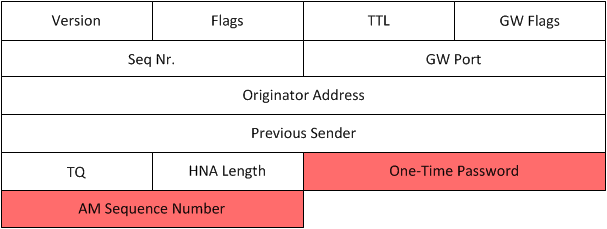
\includegraphics{images/extended_ogm.png}
  	\caption{Modified routing announcement (Originator Message - OGM) for the modified BATMAN protocol.}
	\label{fig:extended_ogm}
\end{figure}

\subsection{POSIX.C}\label{subsect:posix.c}
\subsection{BATMAN.C}
\subsection{SCHEDULE.C}